% Font options: 10pm, 11pt, 12pt
% Align headings left instead of center: nocenter
\documentclass[xcolor=x11names,compress]{beamer}\usepackage[]{graphicx}\usepackage[]{color}
%% maxwidth is the original width if it is less than linewidth
%% otherwise use linewidth (to make sure the graphics do not exceed the margin)
\makeatletter
\def\maxwidth{ %
  \ifdim\Gin@nat@width>\linewidth
    \linewidth
  \else
    \Gin@nat@width
  \fi
}
\makeatother

\definecolor{fgcolor}{rgb}{0.345, 0.345, 0.345}
\newcommand{\hlnum}[1]{\textcolor[rgb]{0.686,0.059,0.569}{#1}}%
\newcommand{\hlstr}[1]{\textcolor[rgb]{0.192,0.494,0.8}{#1}}%
\newcommand{\hlcom}[1]{\textcolor[rgb]{0.678,0.584,0.686}{\textit{#1}}}%
\newcommand{\hlopt}[1]{\textcolor[rgb]{0,0,0}{#1}}%
\newcommand{\hlstd}[1]{\textcolor[rgb]{0.345,0.345,0.345}{#1}}%
\newcommand{\hlkwa}[1]{\textcolor[rgb]{0.161,0.373,0.58}{\textbf{#1}}}%
\newcommand{\hlkwb}[1]{\textcolor[rgb]{0.69,0.353,0.396}{#1}}%
\newcommand{\hlkwc}[1]{\textcolor[rgb]{0.333,0.667,0.333}{#1}}%
\newcommand{\hlkwd}[1]{\textcolor[rgb]{0.737,0.353,0.396}{\textbf{#1}}}%
\let\hlipl\hlkwb

\usepackage{framed}
\makeatletter
\newenvironment{kframe}{%
 \def\at@end@of@kframe{}%
 \ifinner\ifhmode%
  \def\at@end@of@kframe{\end{minipage}}%
  \begin{minipage}{\columnwidth}%
 \fi\fi%
 \def\FrameCommand##1{\hskip\@totalleftmargin \hskip-\fboxsep
 \colorbox{shadecolor}{##1}\hskip-\fboxsep
     % There is no \\@totalrightmargin, so:
     \hskip-\linewidth \hskip-\@totalleftmargin \hskip\columnwidth}%
 \MakeFramed {\advance\hsize-\width
   \@totalleftmargin\z@ \linewidth\hsize
   \@setminipage}}%
 {\par\unskip\endMakeFramed%
 \at@end@of@kframe}
\makeatother

\definecolor{shadecolor}{rgb}{.97, .97, .97}
\definecolor{messagecolor}{rgb}{0, 0, 0}
\definecolor{warningcolor}{rgb}{1, 0, 1}
\definecolor{errorcolor}{rgb}{1, 0, 0}
\newenvironment{knitrout}{}{} % an empty environment to be redefined in TeX

\usepackage{alltt}
%\documentclass[xcolor=x11names,compress,handout]{beamer}
\usepackage[]{graphicx}
\usepackage[]{color}
\usepackage{booktabs}
\usepackage{hyperref}
\usepackage{tikz}
\usepackage{multirow}
\usepackage{multicol}
\usepackage{dcolumn}
\usepackage{bigstrut}
\usepackage{amsmath} 
\usepackage{xcolor,colortbl}
\usepackage{amssymb}
%\newcommand{\done}{\cellcolor{teal}#1}

%% Beamer Layout %%%%%%%%%%%%%%%%%%%%%%%%%%%%%%%%%%
\useoutertheme[subsection=false,shadow]{miniframes}
\useinnertheme{default}
\usefonttheme{serif}
\usepackage{Arev}
\usepackage{pdfpages}

\setbeamerfont{title like}{shape=\scshape}
\setbeamerfont{frametitle}{shape=\scshape, size=\normalsize}

\definecolor{dkblue}{RGB}{0,0,102}

\setbeamercolor*{lower separation line head}{bg=dkblue} 
\setbeamercolor*{normal text}{fg=black,bg=white} 
\setbeamercolor*{alerted text}{fg=red} 
\setbeamercolor*{example text}{fg=black} 
\setbeamercolor*{structure}{fg=black} 
 
\setbeamercolor*{palette tertiary}{fg=black,bg=black!10} 
\setbeamercolor*{palette quaternary}{fg=black,bg=black!10} 

\renewcommand{\(}{\begin{columns}}
\renewcommand{\)}{\end{columns}}
\newcommand{\<}[1]{\begin{column}{#1}}
\renewcommand{\>}{\end{column}}

\setbeamertemplate{navigation symbols}{} 
\setbeamertemplate{footline}[frame number]
\setbeamertemplate{caption}{\raggedright\insertcaption\par}

\setbeamersize{text margin left=5pt,text margin right=5pt}

\AtBeginSection{\frame{\sectionpage}}
\usepackage{xcolor}
\hypersetup{
    colorlinks,
    linkcolor={red!50!black},
    citecolor={blue!50!black},
    urlcolor={blue!80!black}
}

\setbeamercolor{block title}{use=structure,fg=white,bg=structure.fg!75!orange}
\setbeamercolor{block body}{parent=normal text,use=block title,bg=block title.bg!10!bg}

%%%%%%%%%%%%%%%%%%%%%%%%%%%%%%%%%%%%%%%%%%%%%%%%%%




\title{FLS 6441 - Methods III: Explanation and Causation}
\subtitle{Week 2 - A Framework for Explanation}
\author{Jonathan Phillips}
\date{March 2019}
\IfFileExists{upquote.sty}{\usepackage{upquote}}{}
\begin{document}

\frame{\titlepage}

\section{Explanation}

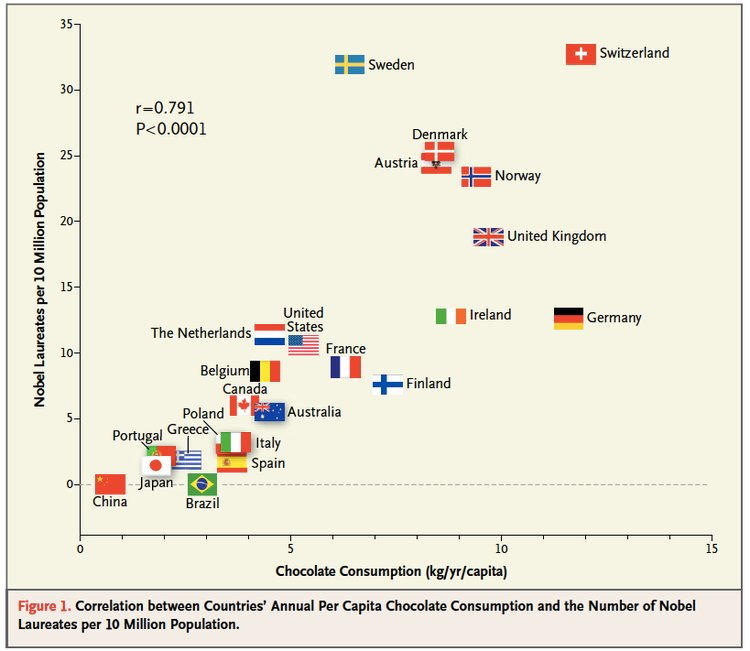
\includegraphics[width=0.9\textwidth]{Chocolate_Nobel.jpg}

\begin{frame}
\frametitle{Explanation}
\small
\begin{itemize}
\item Why isn't correlation enough?
\pause
\begin{itemize}
\item For \textbf{prediction}, correlation is fine: If we know a country has chocolate consumption of 10kg/yr/capita we can reasonably predict it will have about 25 Nobel Laureates
\pause
\item But for \textbf{intervention}, correlation does not help: forcing people to eat more chocolate does nothing on its own to produce more Nobel Laureates
\pause
\item For \textbf{explanation}, correlation also fails - it is no \textit{explanation} to say that Switzerland has the most Nobel Laureates because it has the highest chocolate consumption
\end{itemize}
\end{itemize}
\normalsize
\end{frame}

\begin{frame}
\frametitle{Explanation}
\begin{itemize}
\item What does it mean to explain something?
\pause
\item To give an account of what happens, \textit{and why}
\begin{itemize}
\item The 'chain of causation'
\pause
\end{itemize}
\item If $D$ explains $y$, we are saying that the \textit{absence} of $D$ would have led to a different value of $y$
\pause
\item There exists a 'counterfactual' possibility that did not happen
\end{itemize}
\end{frame}

\begin{frame}
\frametitle{Explanation}
\begin{multicols}{2}
\textcolor{dkblue}{Deterministic Explanation}
\pause
\begin{itemize}
\item \textbf{Sufficient conditions:} Every time $D$ happens, $Y$ happens
\pause
\item \textbf{Necessary conditions:} $Y$ does not happen if $D$ does not happen ('\textit{but for}')
\end{itemize}
\pause
\columnbreak
\textcolor{dkblue}{Probabilistic Explanation}
\pause
\begin{itemize}
\item If $D$ happens, the \textbf{probability} of $Y$ increases
\pause
\item Treatment effects are a distribution, not a single value
\end{itemize}
\end{multicols}
\end{frame}

\begin{frame}
\frametitle{Explanation}
\begin{itemize}
\item Two perspectives on explanation:
\end{itemize}
\pause
\begin{table}[htbp]
  \centering
    \begin{tabular}{|>{\raggedright}p{5cm}|p{5cm}|}
    \toprule
    \textbf{Causes of Effects} & \textbf{Effects of Causes} \\
    \midrule
    What caused Y? & Does D cause Y? \\
    \midrule
    Why does Switzerland have so many Nobel laureates? & Does chocolate cause more Nobel laureates? \\
    \midrule
    Backward-looking & Forward-looking \\
    \bottomrule
    \end{tabular}%
  \label{tab:addlabel}%
\end{table}%
\end{frame}

\begin{frame}
\frametitle{Explanation}
\begin{itemize}
\item Two perspectives on explanation:
\end{itemize}
\begin{multicols}{2}
\begin{knitrout}
\definecolor{shadecolor}{rgb}{0.969, 0.969, 0.969}\color{fgcolor}
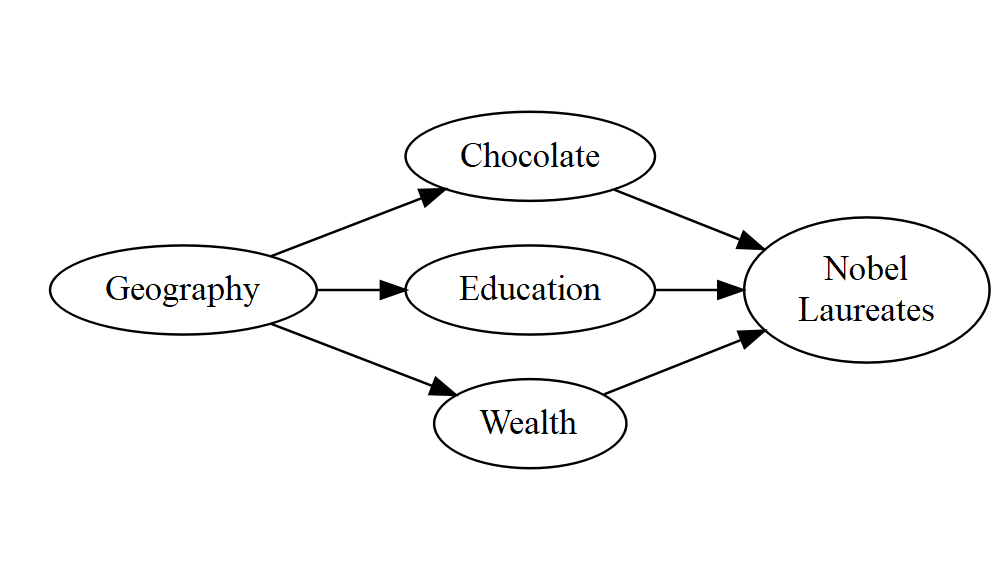
\includegraphics[width=\maxwidth]{figure/explanation1-1} 

\end{knitrout}
\pause
\begin{itemize}
\item Identifying the source of \textbf{ALL} of the variation in Nobel Laureates
\pause
\item An infinite task!
\end{itemize}
\pause
\columnbreak
\begin{knitrout}
\definecolor{shadecolor}{rgb}{0.969, 0.969, 0.969}\color{fgcolor}
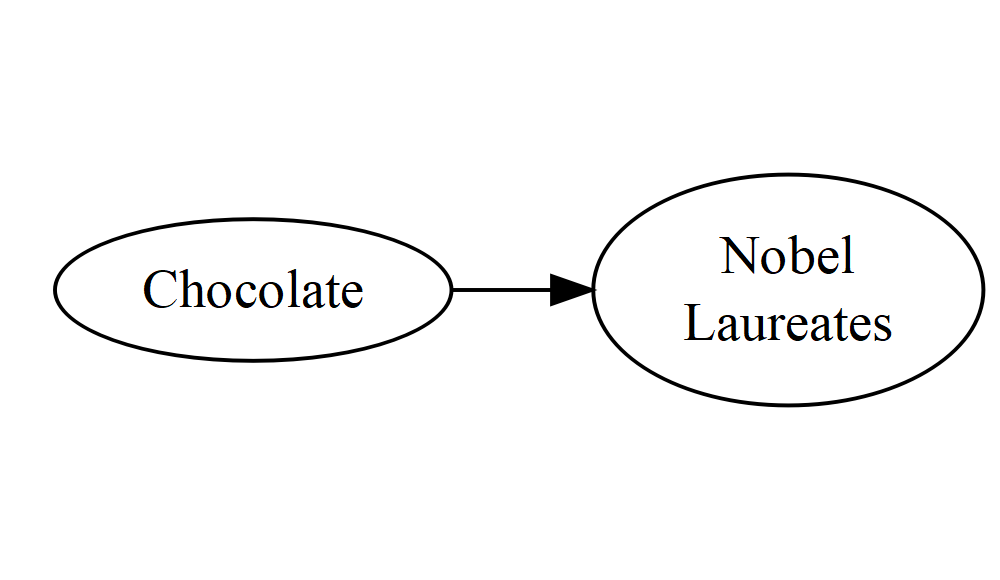
\includegraphics[width=\maxwidth]{figure/explanation2-1} 

\end{knitrout}
\pause
\begin{itemize}
\item Identifying how much \textbf{ONE} variable causes variation in Nobel Laureates
\pause
\item This we can do!
\end{itemize}
\end{multicols}
\end{frame}

\begin{frame}
\frametitle{Explanation}
\begin{itemize}
\item Two perspectives on explanation:
\end{itemize}
\begin{multicols}{2}
\begin{knitrout}
\definecolor{shadecolor}{rgb}{0.969, 0.969, 0.969}\color{fgcolor}
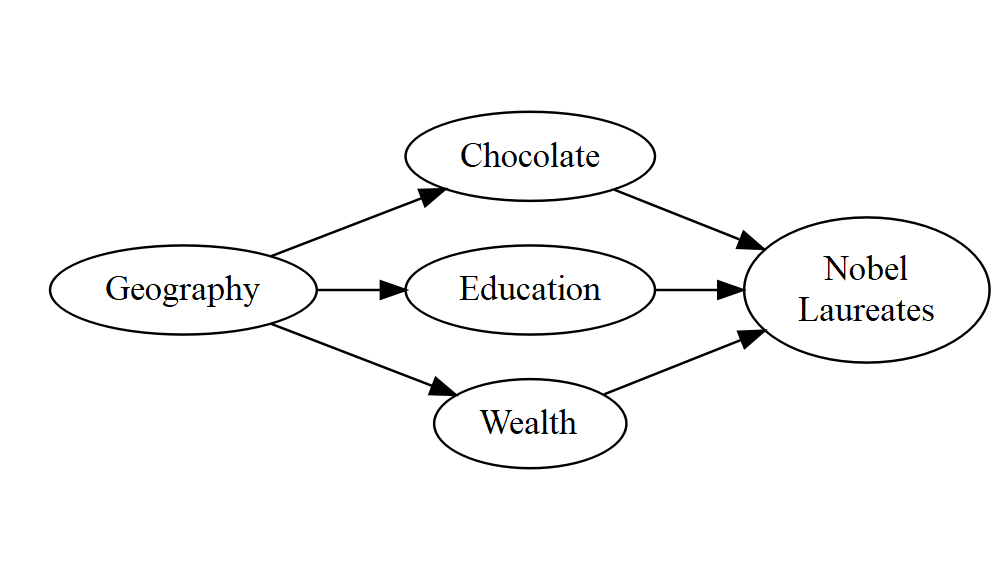
\includegraphics[width=\maxwidth]{figure/explanation1b-1} 

\end{knitrout}
\begin{itemize}
\item Identifying the source of \textbf{ALL} of the variation in Nobel Laureates
\item An infinite task!
\end{itemize}
\columnbreak
\begin{knitrout}
\definecolor{shadecolor}{rgb}{0.969, 0.969, 0.969}\color{fgcolor}
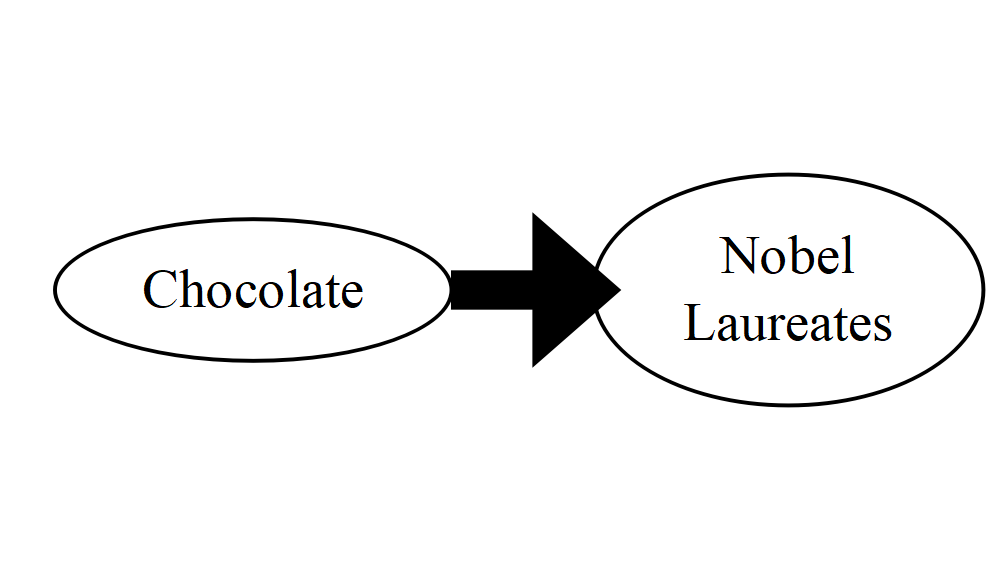
\includegraphics[width=\maxwidth]{figure/explanation2b-1} 

\end{knitrout}
\begin{itemize}
\item Identifying how much \textbf{ONE} variable causes variation in Nobel Laureates
\item This we can do!
\end{itemize}
\end{multicols}
\end{frame}

\begin{frame}
\frametitle{Explanation}
\begin{itemize}
\item Two perspectives on explanation:
\end{itemize}
\begin{multicols}{2}
\begin{knitrout}
\definecolor{shadecolor}{rgb}{0.969, 0.969, 0.969}\color{fgcolor}
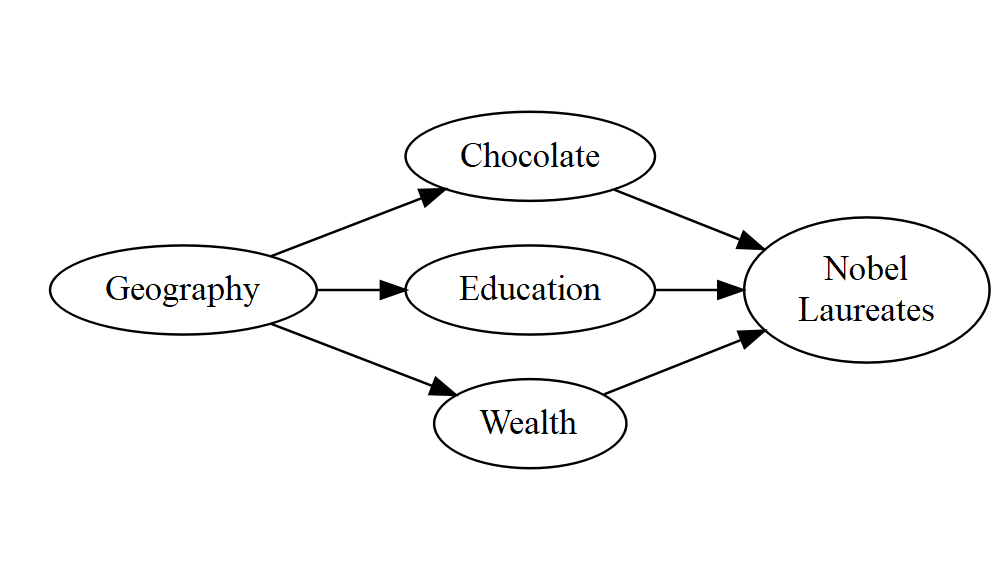
\includegraphics[width=\maxwidth]{figure/explanation1c-1} 

\end{knitrout}
\begin{itemize}
\item Identifying the source of \textbf{ALL} of the variation in Nobel Laureates
\item An infinite task!
\end{itemize}
\columnbreak
\begin{knitrout}
\definecolor{shadecolor}{rgb}{0.969, 0.969, 0.969}\color{fgcolor}
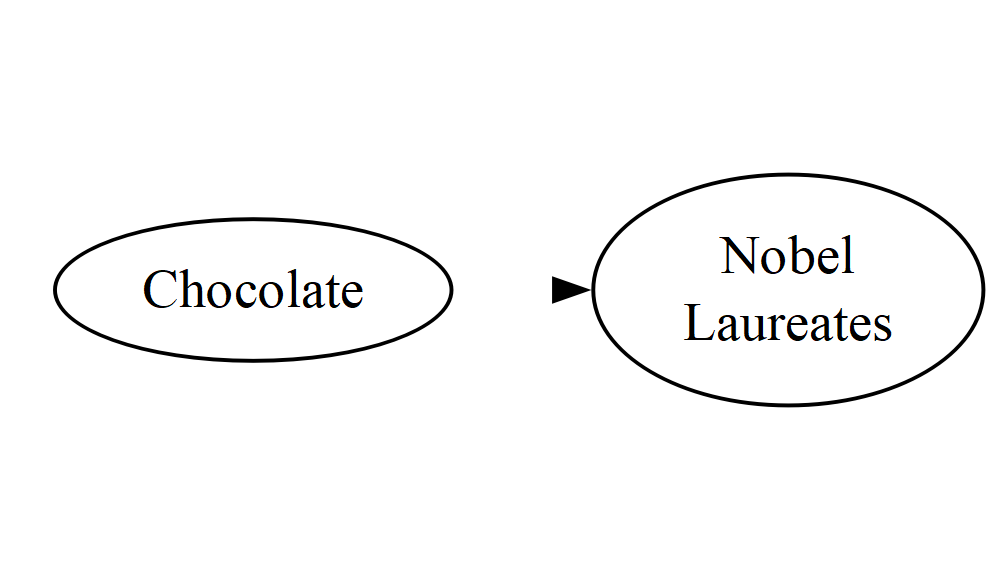
\includegraphics[width=\maxwidth]{figure/explanation2c-1} 

\end{knitrout}
\begin{itemize}
\item Identifying how much \textbf{ONE} variable causes variation in Nobel Laureates
\item This we can do!
\end{itemize}
\end{multicols}
\end{frame}

\begin{frame}
\frametitle{Explanation}
\begin{itemize}
\item A focus on a single explanatory variable $D$ requires a clear definition of \textbf{'Treatment'}
\pause
\item AND to clearly define a \textbf{'Control'}
\pause
\begin{itemize}
\item What is the opposite of investing \$1bn in education?
\pause
\item No investment, or investing it elsewhere?
\pause
\end{itemize}
\item Define treatment:
\end{itemize}
\[D_i = 
\begin{cases}
1 \text{, if treated} \\
0 \text{, if not treated}
\end{cases}
\]
\end{frame}

\begin{frame}
\frametitle{Explanation}
\begin{itemize}
\item Defining our outcome variable:
\pause
\begin{itemize}
\item Is it the outcome we really care about? Or just what's easy to measure?
\pause
\item What theory are we testing?
\end{itemize}
\pause
\item Tempting to look at many outcomes, but the risk of 'cherry-picking'
\pause
\begin{itemize}
\item All outcomes are \textbf{probabilistic} (due to all the other factors we haven't accounted for)
\pause
\item If we study 20 outcomes, on average one will show a significant effect even with no real causal effect
\pause
\end{itemize}
\item So we usually want to study a \textbf{single outcome}
\end{itemize}
\end{frame}

\begin{frame}
\frametitle{Explanation}
\begin{itemize}
\item What are the \textbf{units} of our analysis?
\pause
\begin{itemize}
\item Countries? Political Parties? Individuals?
\pause
\item At what level does causality operate?
\end{itemize}
\pause
\item eg. How does the electoral system affect attitudes to redistribution?
\pause
\begin{itemize}
\item Treatment at the national level
\pause
\item Outcome varies at the individual level
\pause
\item Measurement needed at the lowest (individual) level
\pause
\item But our analysis needs to take account of the 'clustered' treatment
\pause
\end{itemize}
\item Units are \textbf{time-specific}: the same person 10 minutes later is a different unit
\end{itemize}
\end{frame}


\section{Causal Inference}

\begin{frame}
\frametitle{Causal Inference}
\begin{itemize}
\item The \textbf{causal effect} of treatment is how each unit's outcome differs when it is treated and not treated
\pause
\item This means comparing the \textbf{Potential Outcomes} for unit $i$:
\[
Y_{Di} = 
\begin{cases}
Y_{1i}\text{   Potential Outcome if unit i treated} \\
Y_{0i}\text{   Potential Outcome if unit i NOT treated}
\end{cases}
\]
\pause
\item Individual Treatment Effect for unit $i$: $\alpha_i = Y_{1i} - Y_{0i}$
\end{itemize}
\end{frame}

\begin{frame}
\frametitle{Causal Inference}
\begin{itemize}
\item The \textbf{causal effect} of treatment is how each unit's outcome differs when it is treated and not treated
\item This means comparing the \textbf{Potential Outcomes} for unit $i$:
\[
Y_{Di} = 
\begin{cases}
Y_{1i}\text{   GDP Growth of Brazil in 2010 if a Democracy} \\
Y_{0i}\text{   GDP Growth of Brazil in 2010 if NOT a Democracy}
\end{cases}
\]
\item Individual Treatment Effect for unit $i$: $\alpha_i = Y_{1i} - Y_{0i}$
\end{itemize}
\end{frame}

\begin{frame}
\frametitle{Causal Inference}
\begin{itemize}
\item We are explicitly thinking about \textbf{counterfactuals}
\pause
\begin{itemize}
\item What would have happened to the same unit if the treatment had not happened?
\pause
\item What would Brazil's GDP growth rate be if we lived in a dictatorship?
\pause
\item Would World War I still have happened if Archduke Franz Ferdinand had not been assassinated in 1914?
\pause
\item Would Brazil have won the 2014 World Cup if Neymar had not been injured?
\pause
\end{itemize}
\end{itemize}
\end{frame}

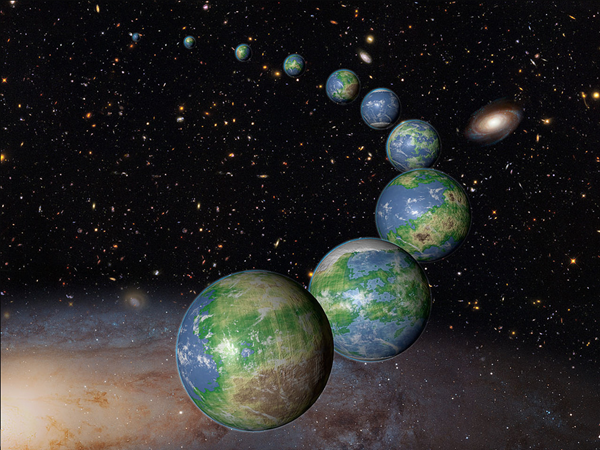
\includegraphics[width=1\textwidth]{figure/Multiverse.png}

\begin{frame}
\frametitle{Causal Inference}
\footnotesize
\begin{table}[htbp]
  \centering
  \caption{Potential Outcomes are just another Variable for each Unit}
    \begin{tabular}{|p{2.4cm}|p{2.4cm}|p{2.4cm}|p{2.4cm}|}
    \hline
          & \multicolumn{1}{p{2.4cm}|}{GDP Growth if Democracy} & \multicolumn{1}{p{2.4cm}|}{GDP Growth if  NOT Democracy} &  Treatment Effect\bigstrut\\
    \hline
          & \multicolumn{1}{l|}{$Y_1$} & \multicolumn{1}{l|}{$Y_0$} & \multicolumn{1}{l|}{$Y_1-Y_0$} \bigstrut\\
    \hline
    Brasil & 4     & 1     & 3 \bigstrut\\
    \hline
    Argentina & 7    & 4     & 3 \bigstrut\\
    \hline
    Bolivia & 2     & 4     & -2 \bigstrut\\
    \hline
    Colombia & 7    & 7    & 0 \bigstrut\\
    \hline
    Peru & 5     & 4     & 1 \bigstrut\\
    \hline
    \end{tabular}%
  \label{tab:addlabel}%
\end{table}%
\normalsize
\end{frame}

\begin{frame}
\frametitle{Causal Inference}
\begin{itemize}
\item Political Science is not about explaining individual events
\pause
\item We ideally want general theories that apply to \textit{all our units}
\pause
\item To explain a systematic treatment - not a single event - we need \textbf{multiple counterfactual comparisons}
\pause
\item We know how democracy works in Europe; the question is what will happen if it becomes more common in the whole world?
\pause
\begin{block}{Average Treatment Effect}
\item We want to calculate an \textbf{Average Treatment Effect} 
\pause 
\item $$ATE=E(\alpha_i) = E (Y_1 - Y_0) = E(Y_1) - E(Y_0) = \frac{\sum_i (Y_{1i} - Y_{0i})}{N}$$
\end{block}
\end{itemize}
\end{frame}

\begin{frame}
\frametitle{Causal Inference}
\footnotesize
\begin{table}[htbp]
  \centering
  \caption{Potential Outcomes are just another Variable for each Unit}
    \begin{tabular}{|p{2.4cm}|p{2.4cm}|p{2.4cm}|p{2.4cm}|}
    \hline
          & \multicolumn{1}{p{2.4cm}|}{GDP Growth if Democracy} & \multicolumn{1}{p{2.4cm}|}{GDP Growth if  NOT Democracy} & Treatment Effect \bigstrut\\
    \hline
          & \multicolumn{1}{p{2.4cm}|}{$Y_1$} & \multicolumn{1}{l|}{$Y_0$} & \multicolumn{1}{l|}{$Y_{1} - Y_{0}$} \bigstrut\\
    \hline
    Brasil & 4     & 1     & 3 \bigstrut\\
    \hline
    Argentina & 7    & 4     & 3 \bigstrut\\
    \hline
    Bolivia & 2     & 4     & -2 \bigstrut\\
    \hline
    Colombia & 7    & 7    & 0 \bigstrut\\
    \hline
    Peru & 5     & 4     & 1 \bigstrut\\
    \hline
    \textbf{Average Treatment Effect} & \textbf{5} & \textbf{4} & \textbf{1} \bigstrut\\
    \hline
    \end{tabular}%
  \label{tab:addlabel}%
\end{table}%
\normalsize
\end{frame}

\begin{frame}
\frametitle{Causal Inference}
\begin{itemize}
\item In reality, some units are \textbf{actually treated} ($D=1$), others are \textbf{actually control} ($D=0$)
\end{itemize}
\pause
\footnotesize
\begin{block}{Average Treatment Effect on the Treated}
\begin{multline}
\item $$ATT=E(\alpha_i|D=1) = E (Y_1 - Y_0|D=1) = \frac{\sum_i (Y_{1i} - Y_{0i}|D=1)}{N_{Treated}}$$
\end{multline}
\end{block}
\pause
\begin{block}{Average Treatment Effect on the Untreated (Control)}
\begin{multline}
\item $$ATU=E(\alpha_i|D=0) = E (Y_1 - Y_0|D=0) = \frac{\sum_i (Y_{1i} - Y_{0i}|D=0)}{N_{Control}}$$
\end{multline}
\end{block}
\normalsize
\pause
\begin{itemize}
\item The three effect estimates are usually different
\begin{itemize}
\item The effect democracy has had in Europe is different to the effect if it were introduced in Africa
\end{itemize}
\end{itemize}
\end{frame}

\begin{frame}
\frametitle{Causal Inference}
\footnotesize
\begin{table}[htbp]
  \centering
  \caption{Potential Outcomes Example}
    \begin{tabular}{|p{1.8cm}|p{1.8cm}|p{2cm}|p{2cm}|p{2cm}|}
    \hline
          & \multicolumn{1}{p{1.8cm}|}{Democracy?} & \multicolumn{1}{p{2cm}|}{GDP Growth if Democracy} & \multicolumn{1}{p{2.2cm}|}{GDP Growth if NOT Democracy} &  Treatment Effect \bigstrut\\
    \hline
          & \multicolumn{1}{p{1.8cm}|}{$D_i$} & \multicolumn{1}{p{2cm}|}{$Y_1$} & \multicolumn{1}{p{2.2cm}|}{$Y_0$} & \multicolumn{1}{p{1.8cm}|}{$Y_{1} - Y_{0}$} \bigstrut\\
    \hline
    Brasil & 1 & 4     & 1      & 3 \bigstrut\\
    \hline
    Argentina & 0 & 7    & 4      & 3 \bigstrut\\
    \hline
    Bolivia & 1 & 2     & 4     & -2 \bigstrut\\
    \hline
    Colombia & 0 &  7   & 7    & 0 \bigstrut\\
    \hline
    Peru & 0 & 5     & 4     & 1 \bigstrut\\
\hline
    \end{tabular}%
  \label{tab:addlabel}%
\end{table}%
\normalsize
\end{frame}

\begin{frame}
\frametitle{Causal Inference}
\footnotesize
\begin{table}[htbp]
  \centering
  \caption{Potential Outcomes Example}
    \begin{tabular}{|p{1.8cm}|p{1.8cm}|p{2cm}|p{2cm}|p{2cm}|}
    \hline
          & \multicolumn{1}{p{1.8cm}|}{Democracy?} & \multicolumn{1}{p{2cm}|}{GDP Growth if Democracy} & \multicolumn{1}{p{2.2cm}|}{GDP Growth if NOT Democracy} &  Treatment Effect \bigstrut\\
    \hline
          & \multicolumn{1}{p{1.8cm}|}{$D_i$} & \multicolumn{1}{p{2cm}|}{$Y_1$} & \multicolumn{1}{p{2.2cm}|}{$Y_0$} & \multicolumn{1}{p{1.8cm}|}{$Y_{1} - Y_{0}$} \bigstrut\\
    \hline
    Brasil & 1 & 4     & 1      & 3 \bigstrut\\
    \hline
     &  &     &       &  \bigstrut\\[-2ex]
    \hline
    Bolivia & 1 & 2     & 4     & -2 \bigstrut\\
    \hline
     &  &     &     &  \bigstrut\\[-2ex]
    \hline
     &  &      &      &  \bigstrut\\[-2ex]
    \hline
    \textbf{ATT} & \textbf{1} & \textbf{3}     & \textbf{2.5}     & \textbf{0.5} \bigstrut\\
\hline
    \end{tabular}%
  \label{tab:addlabel}%
\end{table}%
\normalsize
\end{frame}

\begin{frame}
\frametitle{Causal Inference}
\footnotesize
\begin{table}[htbp]
  \centering
  \caption{Potential Outcomes Example}
    \begin{tabular}{|p{1.8cm}|p{1.8cm}|p{2cm}|p{2cm}|p{2cm}|}
    \hline
          & \multicolumn{1}{p{1.8cm}|}{Democracy?} & \multicolumn{1}{p{2cm}|}{GDP Growth if Democracy} & \multicolumn{1}{p{2.2cm}|}{GDP Growth if NOT Democracy} &  Treatment Effect \bigstrut\\
    \hline
          & \multicolumn{1}{p{1.8cm}|}{$D_i$} & \multicolumn{1}{p{2cm}|}{$Y_1$} & \multicolumn{1}{p{2.2cm}|}{$Y_0$} & \multicolumn{1}{p{1.8cm}|}{$Y_{1} - Y_{0}$} \bigstrut\\
    \hline
     &  &      &       &  \bigstrut\\[-2ex]
    \hline
    Argentina & 0 & 7    & 4      & 3 \bigstrut\\
    \hline
     &  &      &      &  \bigstrut\\[-2ex]
    \hline
    Colombia & 0 &  7   & 7    & 0 \bigstrut\\
    \hline
    Peru & 0 & 5     & 4     & 1 \bigstrut\\
    \hline
    \textbf{ATU} & \textbf{0} & \textbf{6.3}     & \textbf{5}     & \textbf{1.3} \bigstrut\\
\hline
    \end{tabular}%
  \label{tab:addlabel}%
\end{table}%
\normalsize
\end{frame}

\begin{frame}
\frametitle{Causal Inference}
\begin{block}{The Fundamental Problem of Causal Inference}
\begin{itemize}
\item No units can receive \textbf{both} treatment and control
\pause
\item So we can never observe both $Y_1$ and $Y_0$ \textbf{for the same unit}
\pause
\item \textit{Individual} Treatment Effects are \textbf{Impossible to Estimate}
\end{itemize}
\end{block}
\pause
\[
Y_{i}^{obs} = 
\begin{cases}
Y_{1i} \text{ if } D_i=1 \\
Y_{0i} \text{ if } D_i=0
\end{cases}
\]
\pause
$$Y_{i}^{obs} = D_i \cdot Y_{1i} + (1-D_i) \cdot Y_{0i}$$
\end{frame}

\begin{frame}
\frametitle{Causal Inference}
\footnotesize
\begin{table}[htbp]
  \centering
  \caption{Potential Outcomes Example}
    \begin{tabular}{|p{1.8cm}|p{1.8cm}|p{2cm}|p{2cm}|p{2cm}|}
    \hline
          & \multicolumn{1}{p{1.8cm}|}{Democracy?} & \multicolumn{1}{p{2cm}|}{GDP Growth if Democracy} & \multicolumn{1}{p{2.2cm}|}{GDP Growth if NOT Democracy} &  Treatment Effect \bigstrut\\
    \hline
          & \multicolumn{1}{p{1.8cm}|}{$D_i$} & \multicolumn{1}{p{2cm}|}{$Y_1$} & \multicolumn{1}{p{2.2cm}|}{$Y_0$} & \multicolumn{1}{p{1.8cm}|}{$Y_{1} - Y_{0}$} \bigstrut\\
    \hline
    Brasil & 1 & 4     & 1      & 3 \bigstrut\\
    \hline
    Argentina & 0 & 7    & 4      & 3 \bigstrut\\
    \hline
    Bolivia & 1 & 2     & 4     & -2 \bigstrut\\
    \hline
    Colombia & 0 &  7   & 7    & 0 \bigstrut\\
    \hline
    Peru & 0 & 5     & 4     & 1 \bigstrut\\
\hline
    \end{tabular}%
  \label{tab:addlabel}%
\end{table}%
\normalsize
\end{frame}

\begin{frame}
\frametitle{Causal Inference}
\footnotesize
\begin{table}[htbp]
  \centering
  \caption{Potential Outcomes Example}
    \begin{tabular}{|p{1.8cm}|p{1.8cm}|p{2cm}|p{2cm}|p{2cm}|}
    \hline
          & \multicolumn{1}{p{1.8cm}|}{Democracy?} & \multicolumn{1}{p{2cm}|}{GDP Growth if Democracy} & \multicolumn{1}{p{2.2cm}|}{GDP Growth if NOT Democracy} & Treatment Effect \bigstrut\\
    \hline
          & \multicolumn{1}{p{1.8cm}|}{$D_i$} & \multicolumn{1}{p{2cm}|}{$Y_1$} & \multicolumn{1}{p{2.2cm}|}{$Y_0$} & \multicolumn{1}{p{1.8cm}|}{$Y_{1} - Y_{0}$} \bigstrut\\
    \hline
    Brasil & 1 & 4     & ?      & ? \bigstrut\\
    \hline
    Argentina & 0 & ?    & 4      & ? \bigstrut\\
    \hline
    Bolivia & 1 & 2     & ?     & ? \bigstrut\\
    \hline
    Colombia & 0 &  ?   & 7    & ? \bigstrut\\
    \hline
    Peru & 0 & ?     & 4     & ? \bigstrut\\
\hline
    \end{tabular}%
  \label{tab:addlabel}%
\end{table}%
\normalsize
\end{frame}

\begin{frame}
\frametitle{Causal Inference}
\footnotesize
\begin{table}[htbp]
  \centering
  \caption{Potential Outcomes Example}
    \begin{tabular}{|p{1.8cm}|p{1.8cm}|p{2cm}|p{2cm}|p{2cm}|}
    \hline
          & \multicolumn{1}{p{1.8cm}|}{Democracy?} & \multicolumn{1}{p{2cm}|}{GDP Growth if Democracy} & \multicolumn{1}{p{2.2cm}|}{GDP Growth if NOT Democracy} & \textbf{Observed} GDP Growth \bigstrut\\
    \hline
          & \multicolumn{1}{p{1.8cm}|}{$D_i$} & \multicolumn{1}{p{2cm}|}{$Y_1$} & \multicolumn{1}{p{2.2cm}|}{$Y_0$} & \multicolumn{1}{p{1.8cm}|}{$Y^{obs}$} \bigstrut\\
    \hline
    Brasil & 1 & 4     & ?      & 4 \bigstrut\\
    \hline
    Argentina & 0 & ?    & 4      & 4 \bigstrut\\
    \hline
    Bolivia & 1 & 2     & ?     & 2 \bigstrut\\
    \hline
    Colombia & 0 &  ?   & 7    & 7 \bigstrut\\
    \hline
    Peru & 0 & ?     & 4     & 4 \bigstrut\\
    \hline
    \end{tabular}%
  \label{tab:addlabel}%
\end{table}%
\normalsize
\end{frame}

\begin{frame}
\frametitle{Causal Inference}
\footnotesize
\begin{table}[htbp]
  \centering
  \caption{Potential Outcomes Example}
    \begin{tabular}{|p{1.8cm}|p{1.8cm}|p{2cm}|}
    \hline
          & \multicolumn{1}{p{1.8cm}|}{Democracy?} & \textbf{Observed} GDP Growth \bigstrut\\
    \hline
          & \multicolumn{1}{p{1.8cm}|}{$D_i$} & \multicolumn{1}{p{1.8cm}|}{$Y^{obs}$} \bigstrut\\
    \hline
    Brasil & 1 & 4 \bigstrut\\
    \hline
    Argentina & 0      & 4 \bigstrut\\
    \hline
    Bolivia & 1      & 2 \bigstrut\\
    \hline
    Colombia & 0    & 7 \bigstrut\\
    \hline
    Peru & 0 & 4 \bigstrut\\
    \hline
    \end{tabular}%
  \label{tab:addlabel}%
\end{table}%
\normalsize
\end{frame}

\begin{frame}
\frametitle{Causal Inference}
\begin{itemize}
\item Actually, nothing stops us calculating the \textbf{Average Treatment Effect}
\pause
\item The question is, is the ATE accurate?
\pause
\end{itemize}
\footnotesize
\begin{table}[htbp]
  \centering
    \begin{tabular}{|p{1.8cm}|p{1.8cm}|p{2cm}|p{2cm}|p{2cm}|}
    \hline
          & \multicolumn{1}{p{1.8cm}|}{Democracy?} & \multicolumn{1}{p{2cm}|}{GDP Growth if Democracy} & \multicolumn{1}{p{2.2cm}|}{GDP Growth if NOT Democracy} & \textbf{Treatment Effect} \bigstrut\\
    \hline
          & \multicolumn{1}{p{1.8cm}|}{$D_i$} & \multicolumn{1}{p{2cm}|}{$Y_1$} & \multicolumn{1}{p{2.2cm}|}{$Y_0$} & \multicolumn{1}{p{1.8cm}|}{$Y_{1} - Y_{0}$} \bigstrut\\
    \hline
    Brasil & 1 & 4     & 1      & 3 \bigstrut\\
    \hline
    Argentina & 0 & 7    & 4      & 3 \bigstrut\\
    \hline
    Bolivia & 1 & 2     & 4     & -2 \bigstrut\\
    \hline
    Colombia & 0 &  7   & 7    & 0 \bigstrut\\
    \hline
    Peru & 0 & 5     & 4     & 1 \bigstrut\\
    \hline
    \textbf{Average Treatment Effect} & & \textbf{5} & \textbf{4} & \textbf{1} \bigstrut\\
    \hline
    \end{tabular}%
  \label{tab:addlabel}%
\end{table}%
\normalsize
\end{frame}

\begin{frame}
\frametitle{Causal Inference}
\begin{itemize}
\item Actually, nothing stops us calculating the \textbf{Average Treatment Effect}
\item The question is, is the ATE accurate?
\end{itemize}
\footnotesize
\begin{table}[htbp]
  \centering
    \begin{tabular}{|p{1.8cm}|p{1.8cm}|p{2cm}|p{2cm}|p{2cm}|}
    \hline
          & \multicolumn{1}{p{1.8cm}|}{Democracy?} & \multicolumn{1}{p{2cm}|}{GDP Growth if Democracy} & \multicolumn{1}{p{2.2cm}|}{GDP Growth if NOT Democracy} & \textbf{Treatment Effect} \bigstrut\\
    \hline
          & \multicolumn{1}{p{1.8cm}|}{$D_i$} & \multicolumn{1}{p{2cm}|}{$Y_1$} & \multicolumn{1}{p{2.2cm}|}{$Y_0$} & \multicolumn{1}{p{1.8cm}|}{$Y_{1} - Y_{0}$} \bigstrut\\
    \hline
    Brasil & 1 & 4     & ?      & ? \bigstrut\\
    \hline
    Argentina & 0 & ?    & 4      & ? \bigstrut\\
    \hline
    Bolivia & 1 & 2     & ?     & ? \bigstrut\\
    \hline
    Colombia & 0 &  ?   & 7    & ? \bigstrut\\
    \hline
    Peru & 0 & ?     & 4     & ? \bigstrut\\
    \hline
    \textbf{Average Treatment Effect} & & \textbf{3} & \textbf{5} & \textbf{-2} \bigstrut\\
    \hline
    \end{tabular}%
  \label{tab:addlabel}%
\end{table}%
\normalsize
\end{frame}

\begin{frame}
\frametitle{Causal Inference}
\begin{itemize}
\item \textbf{So what went wrong?}
\pause
\item The potential outcomes we \textbf{observe} are a \textbf{biased representation} of the potential outcomes of all the units
\pause
\end{itemize}
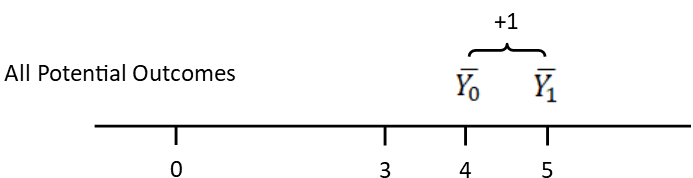
\includegraphics[width=0.9\textwidth]{PO_number_line_1.png}
\end{frame}

\begin{frame}
\frametitle{Causal Inference}
\begin{itemize}
\item \textbf{So what went wrong?}
\item The potential outcomes we \textbf{observe} are a \textbf{biased representation} of the potential outcomes of all the units
\end{itemize}
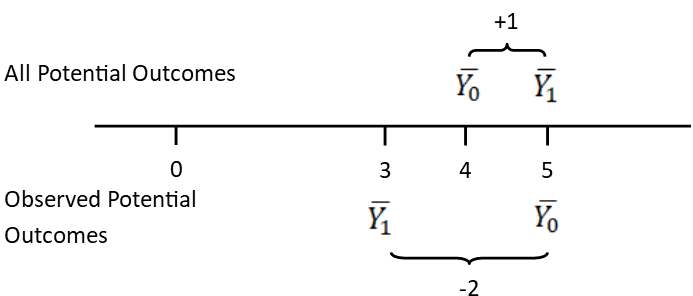
\includegraphics[width=0.9\textwidth]{PO_number_line_2.png}
\begin{itemize}
\item $E(Y_1)$ values are \textbf{biased lower} in the observed data
\pause
\item $E(Y_0)$ values are \textbf{biased higher} in the observed data
\pause
\item So $E(Y_1)-E(Y_0)$ is \textbf{biased}
\end{itemize}
\end{frame}

\begin{frame}
\frametitle{Causal Inference}
\begin{itemize}
\item The Fundamental Problem of Causal Inference means we can only discover causal relationships by comparing \textbf{across units}
\pause
\item Comparing treated $i$ and control $j$ units
\pause
\item If potential outcomes are biased in our observed data:
\pause
\begin{itemize}
\item Our \textbf{counterfactual case $j$} does not represent what would have happened to $i$ in the absence of treatment
\pause
\item Counterfactuals are not \textbf{plausible}
\pause
\item Causal effects are \textbf{biased}
\end{itemize}
\end{itemize}
\end{frame}

\begin{frame}
\frametitle{Causal Inference}
\begin{knitrout}
\definecolor{shadecolor}{rgb}{0.969, 0.969, 0.969}\color{fgcolor}
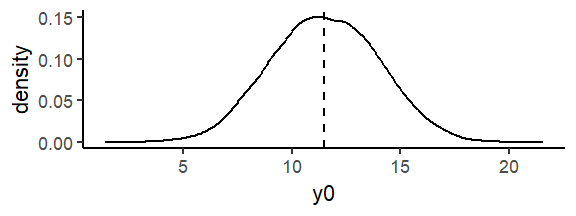
\includegraphics[width=\maxwidth]{figure/OVB1a-1} 

\end{knitrout}
\pause
\begin{knitrout}
\definecolor{shadecolor}{rgb}{0.969, 0.969, 0.969}\color{fgcolor}
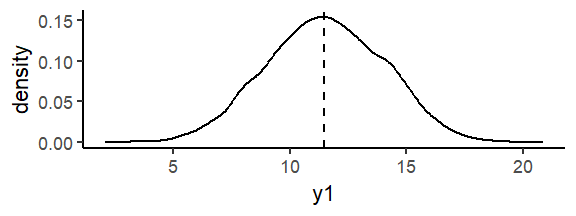
\includegraphics[width=\maxwidth]{figure/OVB2a-1} 

\end{knitrout}
\end{frame}

\begin{frame}
\frametitle{Causal Inference}
\begin{knitrout}
\definecolor{shadecolor}{rgb}{0.969, 0.969, 0.969}\color{fgcolor}
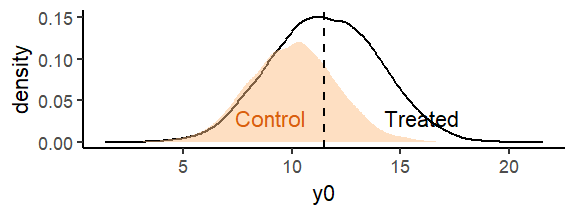
\includegraphics[width=\maxwidth]{figure/OVB1b-1} 

\end{knitrout}

\begin{knitrout}
\definecolor{shadecolor}{rgb}{0.969, 0.969, 0.969}\color{fgcolor}
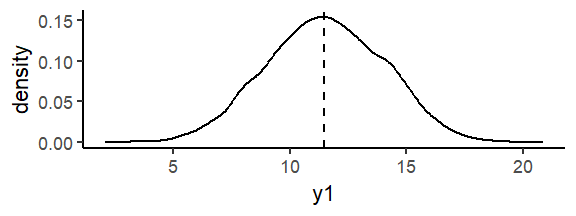
\includegraphics[width=\maxwidth]{figure/OVB2b-1} 

\end{knitrout}
\end{frame}

\begin{frame}
\frametitle{Causal Inference}
\begin{knitrout}
\definecolor{shadecolor}{rgb}{0.969, 0.969, 0.969}\color{fgcolor}
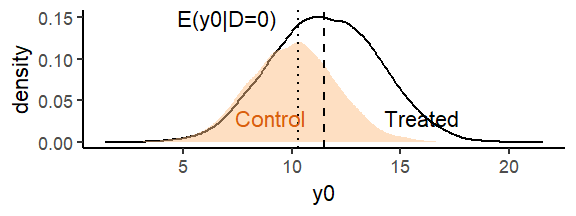
\includegraphics[width=\maxwidth]{figure/OVB1c-1} 

\end{knitrout}

\begin{knitrout}
\definecolor{shadecolor}{rgb}{0.969, 0.969, 0.969}\color{fgcolor}
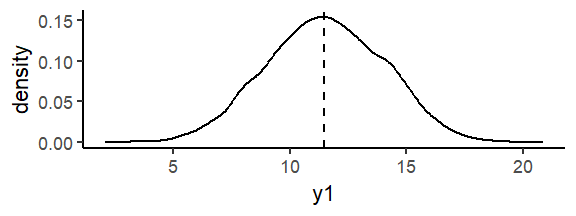
\includegraphics[width=\maxwidth]{figure/OVB2c-1} 

\end{knitrout}
\end{frame}

\begin{frame}
\frametitle{Causal Inference}
\begin{knitrout}
\definecolor{shadecolor}{rgb}{0.969, 0.969, 0.969}\color{fgcolor}
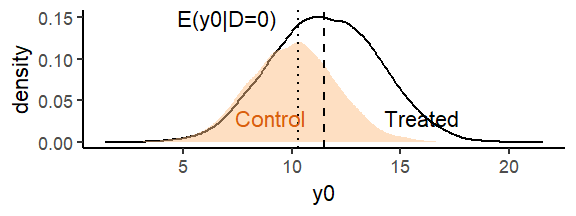
\includegraphics[width=\maxwidth]{figure/OVB1d-1} 

\end{knitrout}

\begin{knitrout}
\definecolor{shadecolor}{rgb}{0.969, 0.969, 0.969}\color{fgcolor}
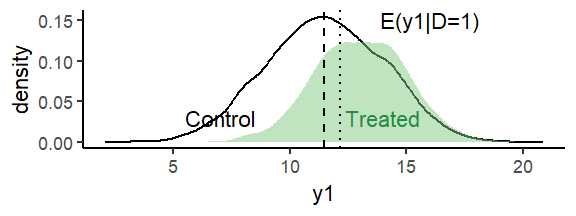
\includegraphics[width=\maxwidth]{figure/OVB2d-1} 

\end{knitrout}
\end{frame}

\begin{frame}
\frametitle{Causal Inference}
\begin{itemize}
\item Lots of averages:
\end{itemize}
\begin{table}[htbp]
  \centering
    \begin{tabular}{|c|l|l|l|}
    \hline
          &       & \multicolumn{2}{c|}{Hypothetical outcome} \bigstrut\\
    \hline
          &       & $Y0$    & $Y1$ \bigstrut\\
    \hline
    \multirow{2}[4]{*}{Actual Treatment} & $D=0$   & $E(Y_{0i}|D=0)$ & $E(Y_{1i}|D=0)$ \bigstrut\\
\cline{2-4}          & $D=1$   & $E(Y_{0i}|D=1)$ & $E(Y_{1i}|D=1)$ \bigstrut\\
    \hline
    \end{tabular}%
  \label{tab:addlabel}%
\end{table}%
\end{frame}

\begin{frame}
\frametitle{Causal Inference}
\begin{itemize}
\item Lots of averages:
\end{itemize}
\begin{table}[htbp]
  \centering
    \begin{tabular}{|c|l|l|l|}
    \hline
          &       & \multicolumn{2}{c|}{Hypothetical outcome} \bigstrut\\
    \hline
          &       & $Y0$    & $Y1$ \bigstrut\\
    \hline
    \multirow{2}[4]{*}{Actual Treatment} & $D=0$   & \cellcolor{blue!25}$E(Y_{0i}|D=0)$ & $E(Y_{1i}|D=0)$ \bigstrut\\
\cline{2-4}          & $D=1$   & $E(Y_{0i}|D=1)$ & \cellcolor{blue!25}$E(Y_{1i}|D=1)$ \bigstrut\\
    \hline
    \end{tabular}%
  \label{tab:addlabel}%
\end{table}%
\end{frame}

\begin{frame}
\frametitle{Causal Inference}
\begin{itemize}
\item All our causal estimates are \textbf{averages}
\pause
\begin{itemize}
\item We cannot distinguish the null hypothesis of no average effect from the sharp null hypothesis of no individual effects
\pause
\end{itemize}
\footnotesize
\begin{table}[htbp]
  \centering
    \begin{tabular}{|l|p{3cm}|p{3cm}|}
    \hline
          & \multicolumn{1}{p{3cm}|}{No Average Effect $E(Y_1-Y_0)=0$} & \multicolumn{1}{p{3cm}|}{"Sharp null": No individual effects ($Y_{1i}-Y_{0i}=0$)} \bigstrut\\
    \hline
    Brasil & 2     & 0 \bigstrut\\
    \hline
    Argentina & -1    & 0 \bigstrut\\
    \hline
    Bolivia & 1     & 0 \bigstrut\\
    \hline
    Colombia & 0     & 0 \bigstrut\\
    \hline
    Peru  & -2    & 0 \bigstrut\\
    \hline
    \textbf{Average} & \textbf{0}     & \textbf{0} \bigstrut\\
    \hline
    \end{tabular}%
  \label{tab:addlabel}%
\end{table}%
\normalsize
\end{itemize}
\end{frame}

\section{Why Observational Data is Biased}

\begin{frame}
\frametitle{Bias}
\begin{itemize}
\item Why are potential outcomes biased in our data?
\pause
\begin{enumerate}
\item Omitted Variables
\pause
\item Reverse Causation
\pause
\item Selection Bias
\pause
\end{enumerate}
\item In all of these cases \textbf{the potential outcomes are distorted}
\pause
\item So basic regression is \textbf{biased}
\end{itemize}
\end{frame}

\begin{frame}
\frametitle{Omitted Variable Bias}
\begin{multicols}{2}
A real causal relationship:
\begin{knitrout}
\definecolor{shadecolor}{rgb}{0.969, 0.969, 0.969}\color{fgcolor}
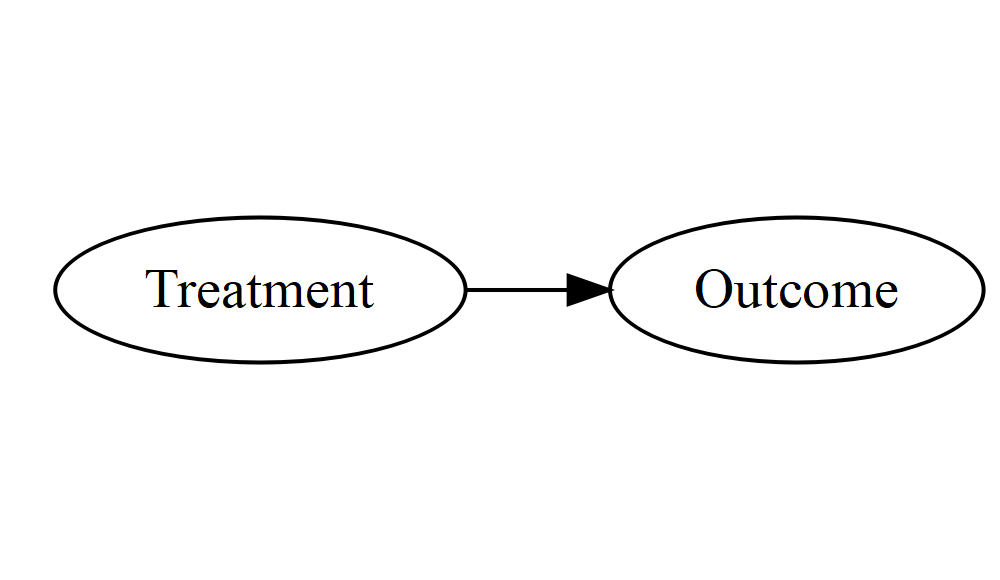
\includegraphics[width=\maxwidth]{figure/explanation3-1} 

\end{knitrout}
\columnbreak
\pause
Being misled by omitted variable bias:
\begin{knitrout}
\definecolor{shadecolor}{rgb}{0.969, 0.969, 0.969}\color{fgcolor}
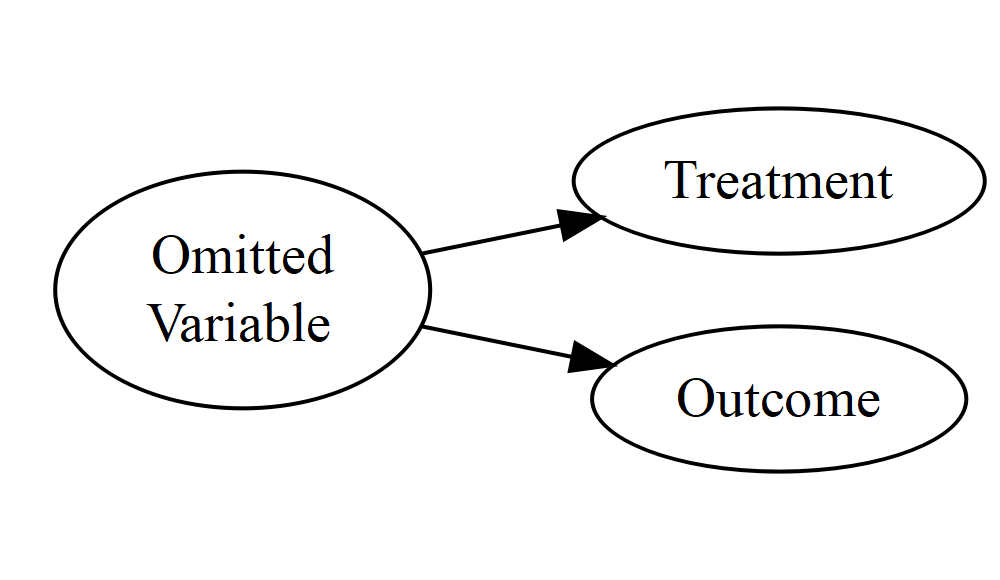
\includegraphics[width=\maxwidth]{figure/explanation4-1} 

\end{knitrout}
\end{multicols}
\begin{itemize}
\pause
\item A third variable causes some units to have \textbf{different values of potential outcomes}, AND for those \textbf{same units to be treated}
\pause
\item So treated units have non-representative $Y_1$
\pause
\item And control units have non-representative $Y_0$
\end{itemize}
\end{frame}

\begin{frame}
\frametitle{Omitted Variable Bias}
\begin{multicols}{2}
A real causal relationship:
\begin{knitrout}
\definecolor{shadecolor}{rgb}{0.969, 0.969, 0.969}\color{fgcolor}
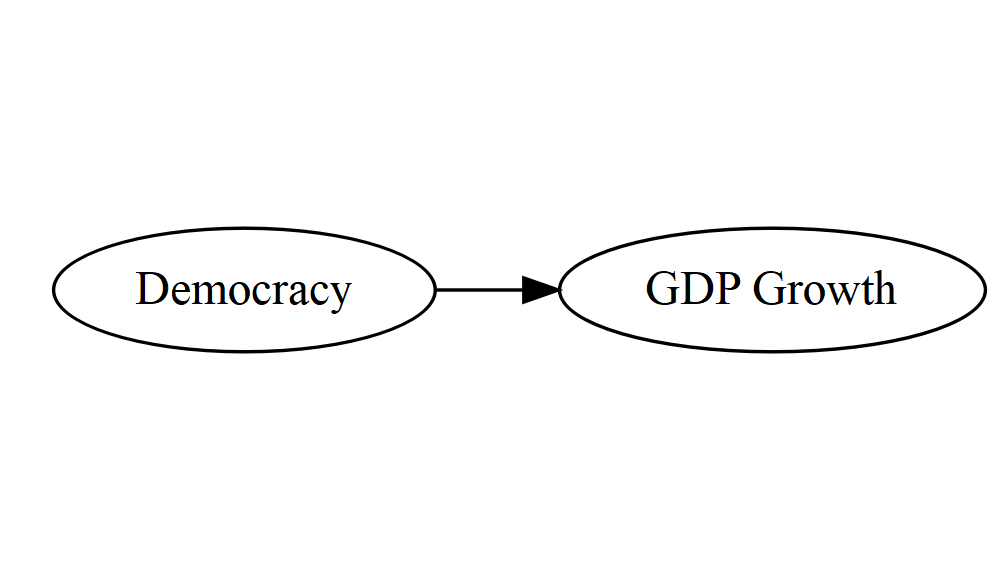
\includegraphics[width=\maxwidth]{figure/explanation9-1} 

\end{knitrout}
\columnbreak
Being misled by omitted variable bias:
\begin{knitrout}
\definecolor{shadecolor}{rgb}{0.969, 0.969, 0.969}\color{fgcolor}
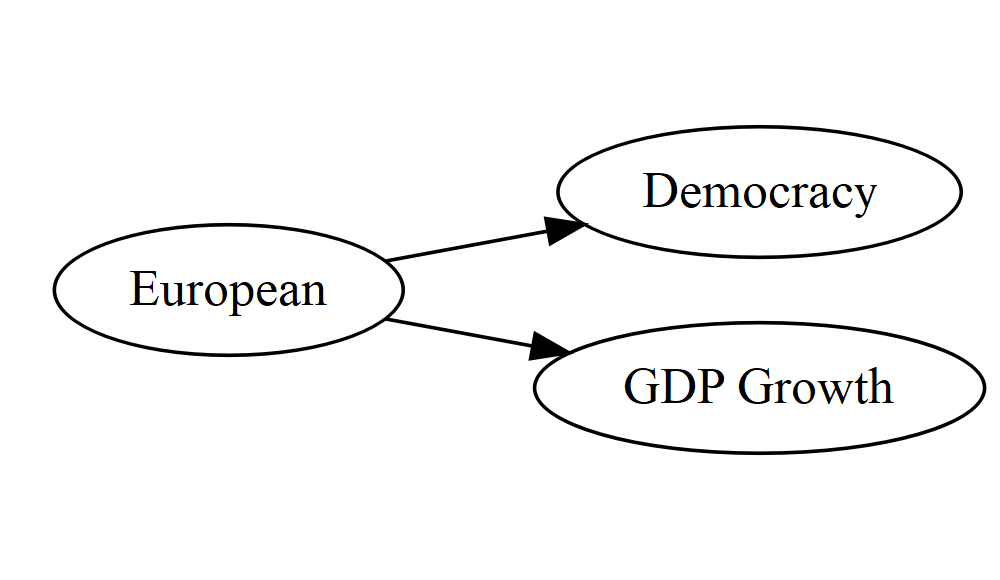
\includegraphics[width=\maxwidth]{figure/explanation10-1} 

\end{knitrout}
\end{multicols}
\begin{itemize}
\pause
\item European countries faced conditions that encouraged both democracy and rapid GDP growth
\end{itemize}
\end{frame}

\begin{frame}
\frametitle{Omitted Variable Bias}
\begin{knitrout}
\definecolor{shadecolor}{rgb}{0.969, 0.969, 0.969}\color{fgcolor}
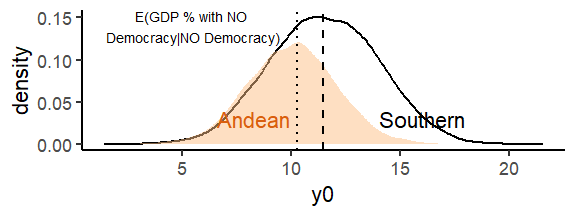
\includegraphics[width=\maxwidth]{figure/OVB3-1} 

\end{knitrout}

\begin{knitrout}
\definecolor{shadecolor}{rgb}{0.969, 0.969, 0.969}\color{fgcolor}
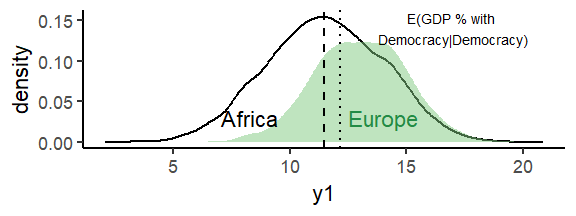
\includegraphics[width=\maxwidth]{figure/OVB4-1} 

\end{knitrout}
\end{frame}

\begin{frame}
\frametitle{Omitted Variable Bias}
\begin{itemize}
\item Let's say that $Y_{1i} = Y_{0i} + \alpha$, where $\alpha$ is the real constant treatment effect
\end{itemize}
$$ \hat{ATE} = E(Y_1|D=1) - E(Y_0|D=0)$$ \\ \pause
$$ \hat{ATE} = \underbrace{\alpha}_\text{Real ATE} + \underbrace{E(Y_0|D=1) - E(Y_0|D=0)}_\text{Bias}$$ \\
\end{frame}


\begin{frame}
\frametitle{Reverse Causation}
\begin{multicols}{2}
A real causal relationship:
\begin{knitrout}
\definecolor{shadecolor}{rgb}{0.969, 0.969, 0.969}\color{fgcolor}
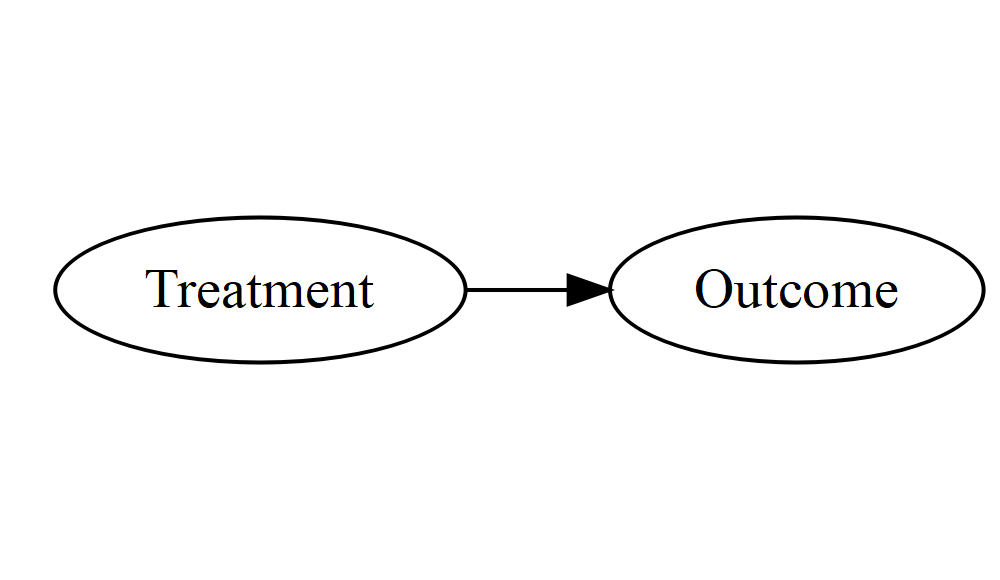
\includegraphics[width=\maxwidth]{figure/explanation5-1} 

\end{knitrout}
\columnbreak
\pause
Being misled by reverse causation:
\begin{knitrout}
\definecolor{shadecolor}{rgb}{0.969, 0.969, 0.969}\color{fgcolor}
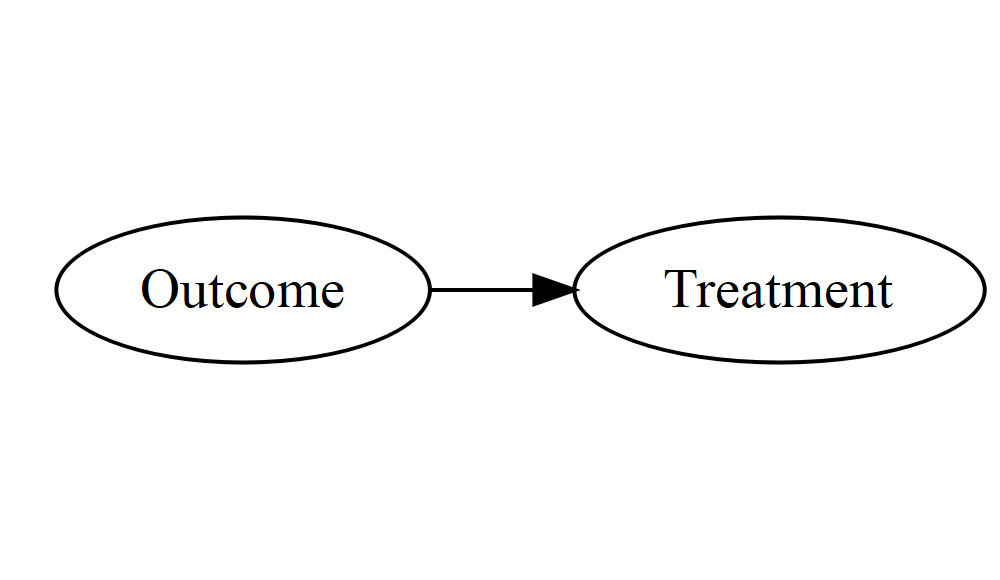
\includegraphics[width=\maxwidth]{figure/explanation6-1} 

\end{knitrout}
\end{multicols}
\begin{itemize}
\pause
\item $D$ does not affect $Y$, but higher $Y$ makes treatment ($D$) more likely
\pause
\item So the two variables are \textbf{correlated}
\end{itemize}
\end{frame}

\begin{frame}
\frametitle{Reverse Causation}
\begin{multicols}{2}
A real causal relationship:
\begin{knitrout}
\definecolor{shadecolor}{rgb}{0.969, 0.969, 0.969}\color{fgcolor}
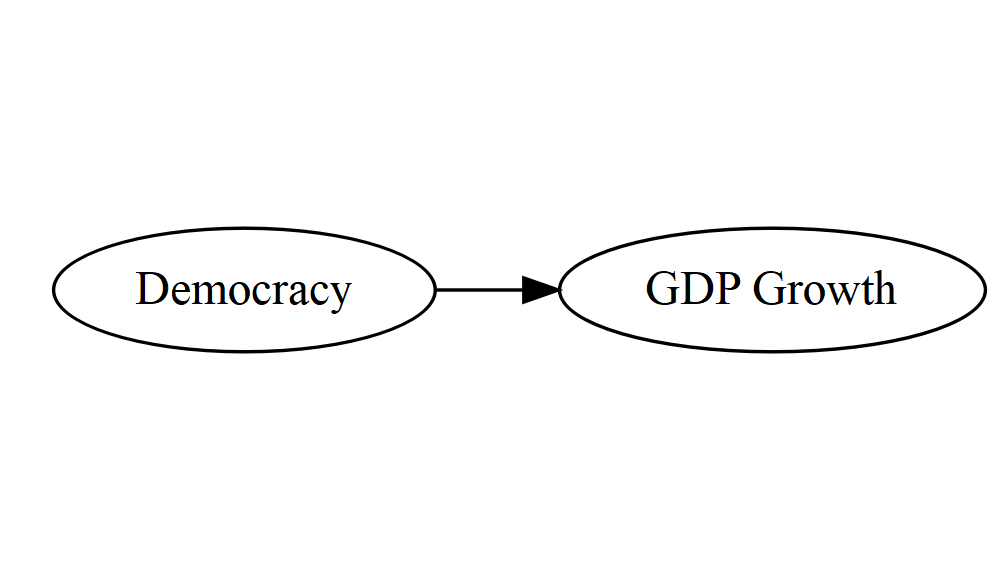
\includegraphics[width=\maxwidth]{figure/reverse1-1} 

\end{knitrout}
\columnbreak
Being misled by reverse causation:
\begin{knitrout}
\definecolor{shadecolor}{rgb}{0.969, 0.969, 0.969}\color{fgcolor}
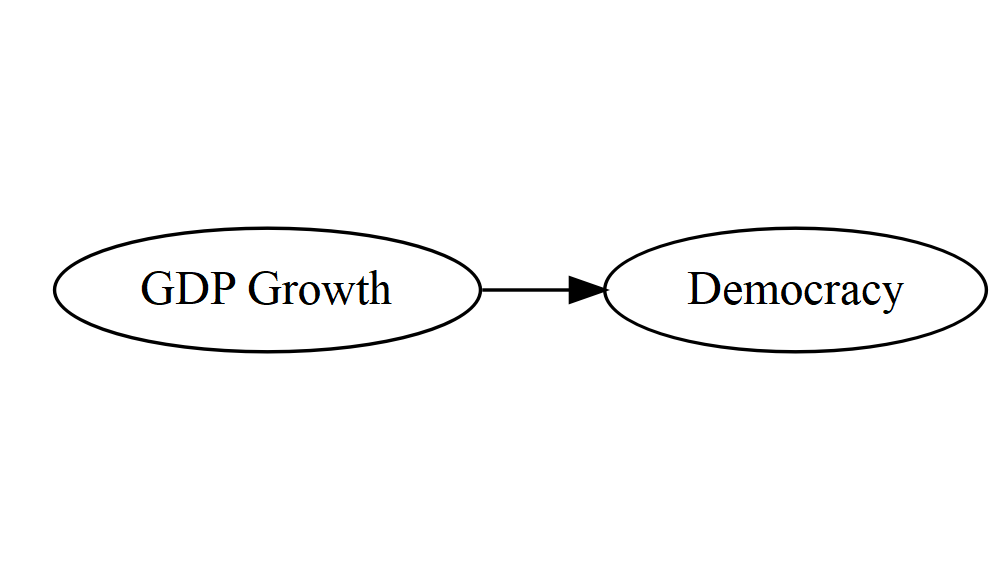
\includegraphics[width=\maxwidth]{figure/reverse2-1} 

\end{knitrout}
\end{multicols}
\begin{itemize}
\pause
\item GDP Growth encourages democratization
\pause
\item So democracies are more likely to have experienced high growth rates
\end{itemize}
\end{frame}

\begin{frame}
\frametitle{Reverse Causation}
\begin{knitrout}
\definecolor{shadecolor}{rgb}{0.969, 0.969, 0.969}\color{fgcolor}
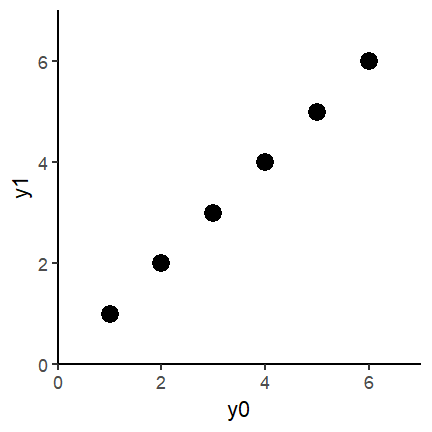
\includegraphics[width=\maxwidth]{figure/reverse3-1} 

\end{knitrout}
\begin{itemize}
\item $E(Y_1-Y_0) = 0$
\end{itemize}
\end{frame}

\begin{frame}
\frametitle{Reverse Causation}
\begin{knitrout}
\definecolor{shadecolor}{rgb}{0.969, 0.969, 0.969}\color{fgcolor}
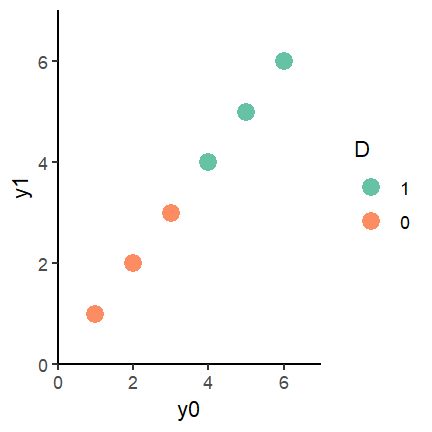
\includegraphics[width=\maxwidth]{figure/reverse5-1} 

\end{knitrout}
\end{frame}

\begin{frame}
\frametitle{Reverse Causation}
\begin{knitrout}
\definecolor{shadecolor}{rgb}{0.969, 0.969, 0.969}\color{fgcolor}
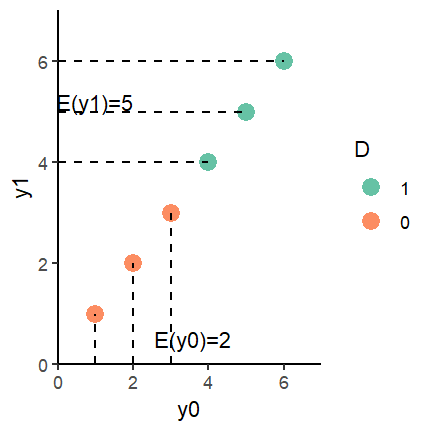
\includegraphics[width=\maxwidth]{figure/reverse6-1} 

\end{knitrout}
\begin{itemize}
\pause
\item $E(Y_1|D=1)-E(Y_0|D=0) = 5 - 2 = 3$
\end{itemize}
\end{frame}

\begin{frame}
\frametitle{Selection Bias}
\begin{multicols}{2}
A real causal relationship:
\begin{knitrout}
\definecolor{shadecolor}{rgb}{0.969, 0.969, 0.969}\color{fgcolor}
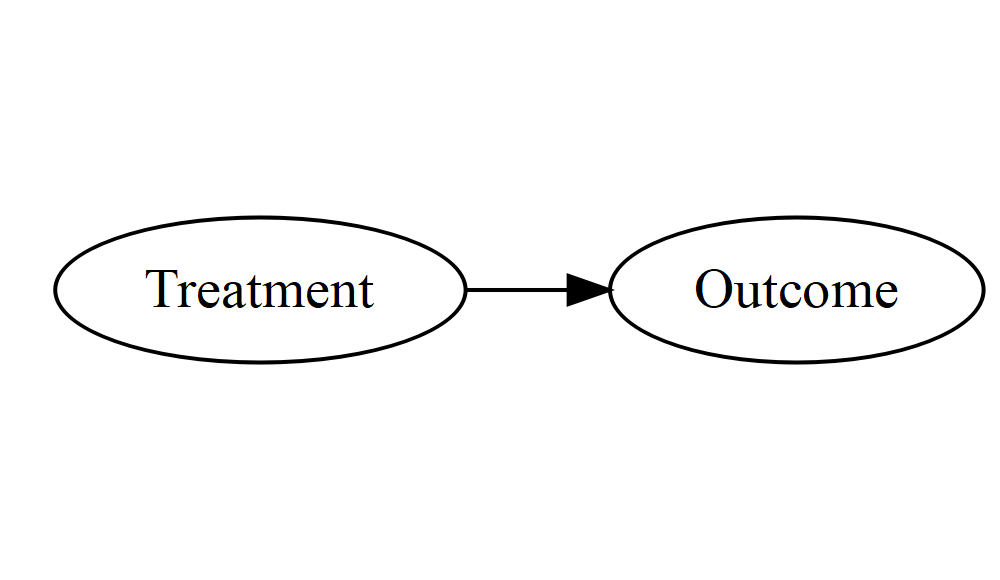
\includegraphics[width=\maxwidth]{figure/explanation7-1} 

\end{knitrout}
\columnbreak
Being misled by Selection Bias:
\begin{knitrout}
\definecolor{shadecolor}{rgb}{0.969, 0.969, 0.969}\color{fgcolor}
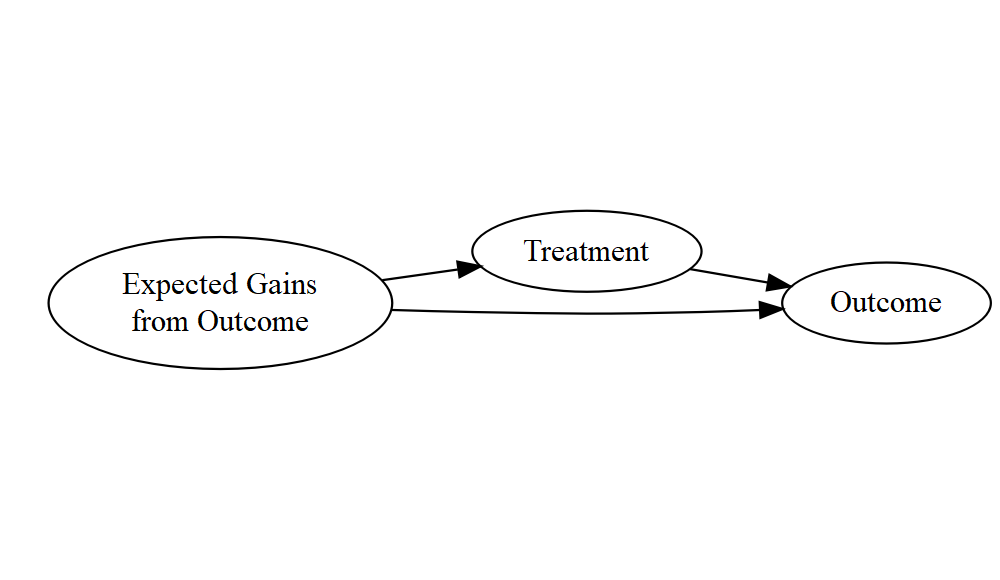
\includegraphics[width=\maxwidth]{figure/explanation8-1} 

\end{knitrout}
\end{multicols}
\end{frame}

\begin{frame}
\frametitle{Selection Bias}
\begin{multicols}{2}
A real causal relationship:
\begin{knitrout}
\definecolor{shadecolor}{rgb}{0.969, 0.969, 0.969}\color{fgcolor}
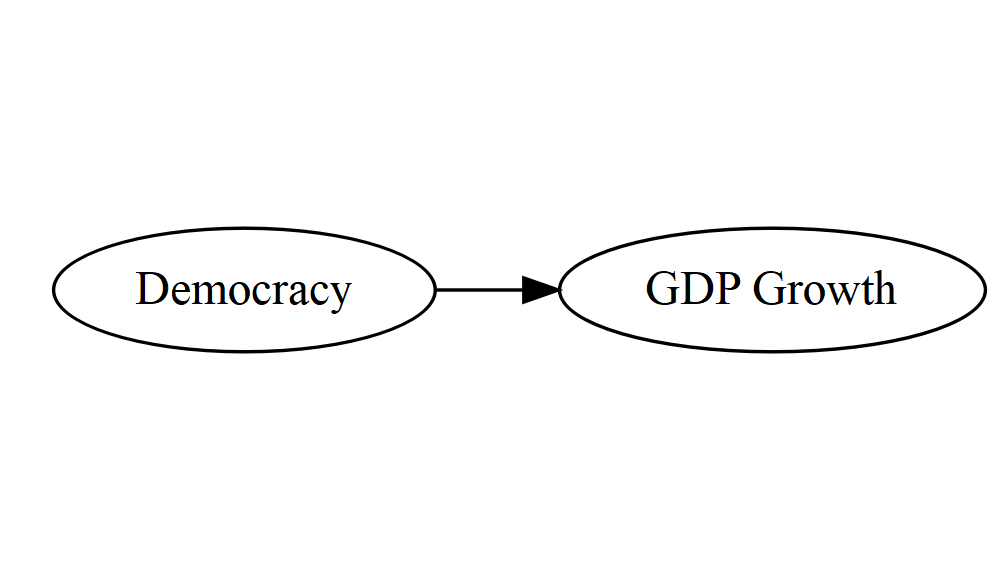
\includegraphics[width=\maxwidth]{figure/explanation9b-1} 

\end{knitrout}
\columnbreak
Being misled by Selection Bias:
\begin{knitrout}
\definecolor{shadecolor}{rgb}{0.969, 0.969, 0.969}\color{fgcolor}
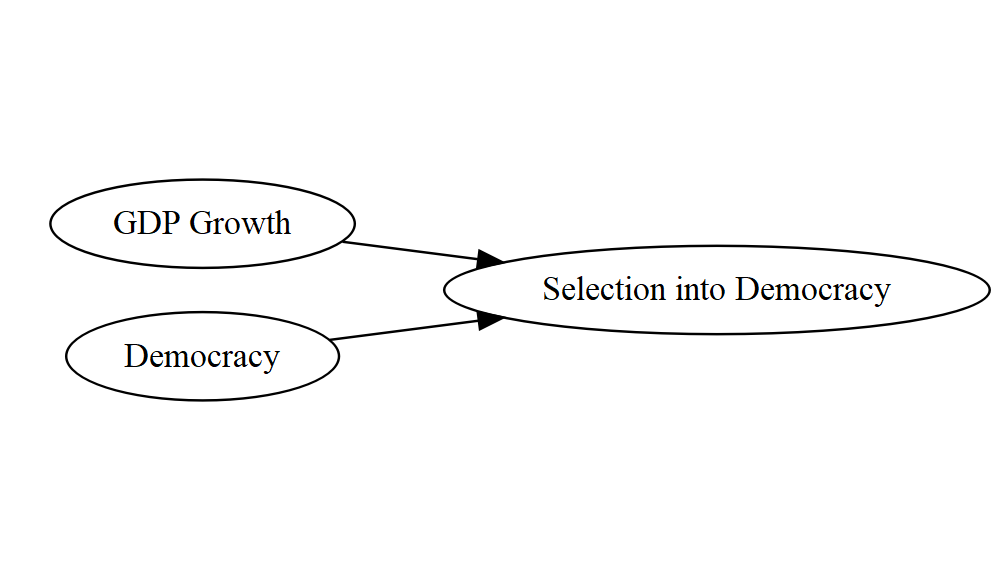
\includegraphics[width=\maxwidth]{figure/explanation10b-1} 

\end{knitrout}
\end{multicols}
\begin{itemize}
\pause
\item The units which benefit most from treatment (largest $y_1-y_0$) \textbf{choose treatment}
\pause
\item We don't see any of the low $y_1$'s of units which avoid treatment
\begin{itemize}
\pause
\item Countries which can boost their GDP growth by becoming a democracy choose to democratize
\pause
\item Ex. Mexico? Myanmar?
\end{itemize}
\end{itemize}
\end{frame}

\begin{frame}
\frametitle{Self-Selection Bias}
\begin{knitrout}
\definecolor{shadecolor}{rgb}{0.969, 0.969, 0.969}\color{fgcolor}
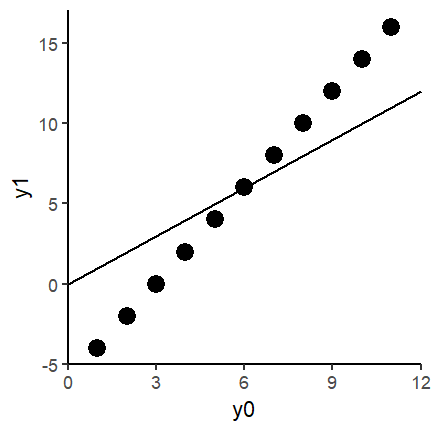
\includegraphics[width=\maxwidth]{figure/SSB1-1} 

\end{knitrout}
\end{frame}

\begin{frame}
\frametitle{Self-Selection Bias}
\begin{knitrout}
\definecolor{shadecolor}{rgb}{0.969, 0.969, 0.969}\color{fgcolor}
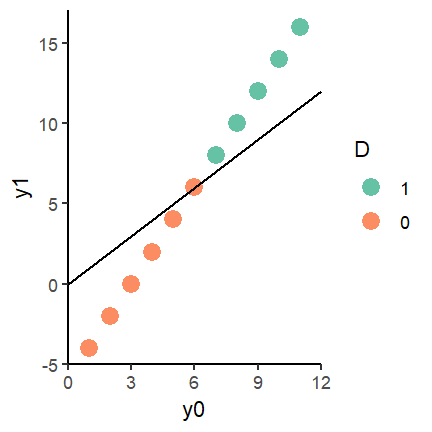
\includegraphics[width=\maxwidth]{figure/SSB2-1} 

\end{knitrout}
\begin{itemize}
\item $E(y_1)-E(y_0)=0$
\end{itemize}
\end{frame}

\begin{frame}
\frametitle{Self-Selection Bias}
\begin{knitrout}
\definecolor{shadecolor}{rgb}{0.969, 0.969, 0.969}\color{fgcolor}
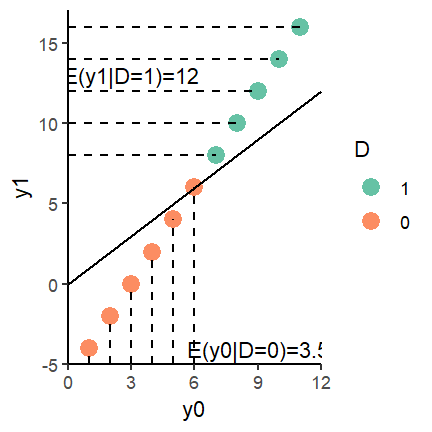
\includegraphics[width=\maxwidth]{figure/SSB3-1} 

\end{knitrout}
\begin{itemize}
\item $E(y_1|D=1)-E(y_0|D=0)=8.5$
\end{itemize}
\end{frame}

\begin{frame}
\frametitle{Self-Selection Bias}
\begin{itemize}
\item Allow treatment effects to vary across individuals, so $Y_{1i} = Y_{0i} + \alpha_i$
\end{itemize}
\pause
\begin{multline}
\underbrace{E(Y_i|D=1)-E(Y_i|D=0)}_\text{Observed Effect} \pause = \underbrace{E(Y_{1i} - Y_{0i})}_\text{Real ATE} \\ + \underbrace{\frac{1}{2}\Big[ E(Y_{1i}|D=1) - E(Y_{1i}|D=0) \Big]}_\text{Imbalance on $Y_1$} + \underbrace{\frac{1}{2}\Big[ E(Y_{0i}|D=1) - E(Y_{0i}|D=0) \Big]}_\text{Imbalance on $Y_0$}
\end{multline}
\footnotesize
NB: For equal-sized treatment and control groups
\normalsize
\end{frame}

\begin{frame}
\frametitle{Treatment Assignment Mechanism}
\begin{itemize}
\item In all of these cases, \textbf{which units receive 'treatment' ($D_i=1$)}, and why, affect our estimate of the relationship between $D$ and $Y$
\pause
\begin{itemize}
\item This is the \textbf{Treatment Assignment Mechanism}
\pause
\end{itemize}
\item Messy treatment assignment mechanisms are why basic regression is no use for explanation
\pause
\begin{itemize}
\item It means our comparison control cases are really misleading
\pause
\item $Y_0$ for North Korea is not a good guide to the $Y_0$ for Sweden
\pause
\item What would happen if the control units got treated?
\end{itemize}
\end{itemize}
\end{frame}


\begin{frame}
\frametitle{Treatment Assignment Mechanism}
\begin{itemize}
\item The comparability of treatment and control units depends on how they got to be treated
\pause
\begin{block}{Treatment Assignment Mechanism}
\item The set of factors that determine why some units have $D=0$ and others have $D=1$
\end{block}
\end{itemize}
\end{frame}

\begin{frame}
\frametitle{Treatment Assignment Mechanism}
\begin{itemize}
\item Explanation is more reliable where the \textbf{Treatment Assignment Mechanism is Independent of Potential Outcomes}
\pause
\begin{itemize}
\item Independent means the values of the potential outcomes give us no information about whether that unit was treated
\pause
\item Potential outcomes are 'balanced' across control and treatment groups
\pause
\end{itemize}
\end{itemize}
\begin{block}{Independence of Treatment Assignment}
\item Treatment Assignment does NOT depend on the values of units' Potential Outcomes
\pause 
\item $(Y_1,Y_0) \perp D$
\pause
\item $Pr(D|(Y_1,Y_0)) = Pr(D)$
\pause
\item $E(Y|D=1) = E(Y|D=0) = E(Y)$
\end{block}
\end{frame}

\begin{frame}
\frametitle{Summary}
\begin{itemize}
\item Template to analyze a paper:
\begin{enumerate}
\item What are the treatment and outcome variables?
\pause
\item What are the Potential Outcomes?
\pause
\item What is the Fundamental Problem of Causal Inference in this case?
\pause
\item How do we define the Average Treatment Effect (ATE) in this case? ATT? ATU?
\pause
\item What is the Treatment Assignment Mechanism?
\pause
\item Draw a causal diagram of the variables in the study, including the treatment assignment mechanism
\pause
\item Is Treatment Assignment independent of Potential Outcomes?
\pause
\item Describe the risk of:
\begin{itemize}
\item Omitted Variable Bias?
\pause
\item Reverse Causation?
\pause
\item Self-Selection?
\end{itemize}
\end{enumerate}
\end{itemize}
\end{frame}

\setbeamercolor{background canvas}{bg=}
\includepdf[pages={2}]{Ross_2001.pdf}

\begin{frame}
\frametitle{Summary}
\begin{itemize}
\item Try experimenting with the \href{https://poliong.shinyapps.io/DAGs/}{Causal Relationships App here}
\pause
\item Can you create an artificial effect between $D$ and $Y$ even when there is no direct causal effect?
\pause
\item Under what conditions can you recover the real treatment effect?
\end{itemize}
\end{frame}

\section{Rest of the Course}

\begin{frame}
\frametitle{Rest of the Course}
\begin{itemize}
\item The rest of the course is mostly about:
\begin{itemize}
\item \textbf{Design-Based Solutions} to the Fundamental Problem of Causal Inference: Which treatment assignment mechanisms \textbf{avoid these biases} and provide plausible counterfactuals
\pause
\item How much can we learn with better research design?
\pause
\item \textbf{Model-Based Solutions:} Not so much.
\end{itemize}
\end{itemize}
\end{frame}

\begin{frame}
\frametitle{Rest of the Course}
\footnotesize
\begin{table}[htbp]
  \centering
  \scalebox{0.7}{
    \begin{tabular}{|p{2.2cm}|p{5cm}|c|c|}
    \hline
          &       & \multicolumn{1}{p{2.4cm}|}{\textbf{Independence of Treatment Assignment}} & \multicolumn{1}{p{3cm}|}{\textbf{Researcher Controls Treatment Assignment?}} \bigstrut\\
    \hline
    \multicolumn{1}{|p{2.8cm}|}{\multirow{2}[4]{2cm}{\textbf{Controlled Experiments}}} & Field Experiments & \checkmark      & \checkmark  \bigstrut\\
\cline{2-4}          & Survey and Lab Experiments &  \checkmark     & \checkmark \bigstrut\\
    \hline
          &       &       &  \bigstrut\\
    \hline
    \multicolumn{1}{|p{2.8cm}|}{\multirow{3}[6]{2cm}{\textbf{Natural Experiments}}} & Randomized Natural Experiments &  \checkmark     &  \bigstrut\\
\cline{2-4}          & Instrumental Variables & \checkmark      &  \bigstrut\\
\cline{2-4}          & Discontinuities & \checkmark      &  \bigstrut\\
    \hline
          &       &       &  \bigstrut\\
    \hline
    \multicolumn{1}{|p{2.8cm}|}{\multirow{4}[8]{2cm}{\textbf{Observational Studies}}} & Difference-in-Differences &       &  \bigstrut\\
\cline{2-4}          & Controlling for Confounding &       &  \bigstrut\\
\cline{2-4}          & Matching &       &  \bigstrut\\
\cline{2-4}          & Comparative Cases and Process Tracing &       &  \bigstrut\\
    \hline
    \end{tabular}}%
  \label{tab:addlabel}%
\end{table}%
\normalsize
\end{frame}

\end{document}


%setwd('C:\\Users\\Jonny\\Google Drive\\Academic\\USP\\Class\\Week 1 - Intro\\Lecture Slides')
%knitr::knit("Slides_Wk1_intro_5.Rnw")
